% Notable deployments of the five-role decomposition, redrawn from
% Casadei et al. (2020), Figure 4. Solid boxes are hosts (thick border: thick
% host, thin border: thin host); dotted boxes are components, one colour per
% logical device. Colours and link styles match pulverisation-components.tex.
% Input inside a figure environment: styles stay local to it.
\colorlet{pdA}{blue!18}
\colorlet{pdB}{red!18}
\colorlet{pdC}{green!25}
\colorlet{pdD}{gray!40}
\tikzset{
  pdcomp/.style={draw,densely dotted,fill=#1,minimum size=4mm,inner sep=0pt,font=\footnotesize},
  thickhost/.style={draw,line width=1.1pt,fill=gray!12},
  thinhost/.style={draw,line width=0.4pt,fill=gray!12},
  hostlink/.style={line width=0.8pt},
  neighbourlink/.style={red!75!black,densely dotted,line width=1pt},
}
\begin{subfigure}[b]{0.48\textwidth}
  \centering
  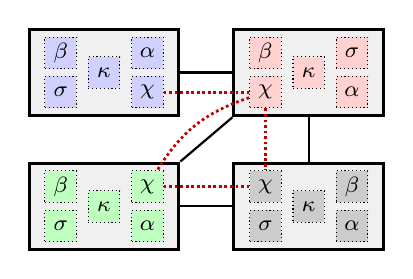
\begin{tikzpicture}
    \node[thickhost,minimum width=19mm,minimum height=11mm] (h1) at (0,0) {};
    \node[thickhost,minimum width=19mm,minimum height=11mm] (h2) at (2.6,0) {};
    \node[thickhost,minimum width=19mm,minimum height=11mm] (h3) at (0,-1.7) {};
    \node[thickhost,minimum width=19mm,minimum height=11mm] (h4) at (2.6,-1.7) {};
    \draw[hostlink] (h1.east) -- (h2.west);
    \draw[hostlink] (h3.east) -- (h4.west);
    \draw[hostlink] (h2.south west) -- (h3.north east);
    \draw[hostlink] (h2.south) -- (h4.north);
    % device A
    \node[pdcomp=pdA] at (-0.55,0.25) {$\beta$};
    \node[pdcomp=pdA] at (-0.55,-0.25) {$\sigma$};
    \node[pdcomp=pdA] at (0,0) {$\kappa$};
    \node[pdcomp=pdA] at (0.55,0.25) {$\alpha$};
    \node[pdcomp=pdA] (c1) at (0.55,-0.25) {$\chi$};
    % device B
    \node[pdcomp=pdB] at (2.05,0.25) {$\beta$};
    \node[pdcomp=pdB] (c2) at (2.05,-0.25) {$\chi$};
    \node[pdcomp=pdB] at (2.6,0) {$\kappa$};
    \node[pdcomp=pdB] at (3.15,0.25) {$\sigma$};
    \node[pdcomp=pdB] at (3.15,-0.25) {$\alpha$};
    % device C
    \node[pdcomp=pdC] at (-0.55,-1.45) {$\beta$};
    \node[pdcomp=pdC] at (-0.55,-1.95) {$\sigma$};
    \node[pdcomp=pdC] at (0,-1.7) {$\kappa$};
    \node[pdcomp=pdC] (c3) at (0.55,-1.45) {$\chi$};
    \node[pdcomp=pdC] at (0.55,-1.95) {$\alpha$};
    % device D
    \node[pdcomp=pdD] (c4) at (2.05,-1.45) {$\chi$};
    \node[pdcomp=pdD] at (2.05,-1.95) {$\sigma$};
    \node[pdcomp=pdD] at (2.6,-1.7) {$\kappa$};
    \node[pdcomp=pdD] at (3.15,-1.45) {$\beta$};
    \node[pdcomp=pdD] at (3.15,-1.95) {$\alpha$};
    % logical neighbourhood
    \draw[neighbourlink] (c1) -- (c2);
    \draw[neighbourlink] (c2) to[bend right=20] (c3);
    \draw[neighbourlink] (c2) -- (c4);
    \draw[neighbourlink] (c3) -- (c4);
  \end{tikzpicture}
  \caption{Peer-to-peer}
  \label{fig:pulverisation-deployments-p2p}
\end{subfigure}\hfill
\begin{subfigure}[b]{0.48\textwidth}
  \centering
  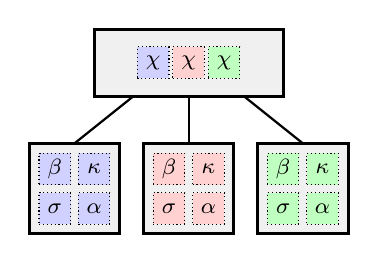
\begin{tikzpicture}
    \node[thickhost,minimum width=24mm,minimum height=8.5mm] at (1.3,0) {};
    \node[pdcomp=pdA] at (0.85,0) {$\chi$};
    \node[pdcomp=pdB] at (1.3,0) {$\chi$};
    \node[pdcomp=pdC] at (1.75,0) {$\chi$};
    \foreach \x/\c/\t in {-0.15/pdA/0.6, 1.3/pdB/1.3, 2.75/pdC/2.0} {
      \draw[hostlink] (\t,-0.425) -- (\x,-1.025);
      \node[thickhost,minimum width=11.5mm,minimum height=11.5mm] at (\x,-1.6) {};
      \node[pdcomp=\c] at (\x-0.25,-1.35) {$\beta$};
      \node[pdcomp=\c] at (\x+0.25,-1.35) {$\kappa$};
      \node[pdcomp=\c] at (\x-0.25,-1.85) {$\sigma$};
      \node[pdcomp=\c] at (\x+0.25,-1.85) {$\alpha$};
    }
  \end{tikzpicture}
  \caption{Broker-based}
  \label{fig:pulverisation-deployments-broker}
\end{subfigure}

\medskip
\begin{subfigure}[b]{0.48\textwidth}
  \centering
  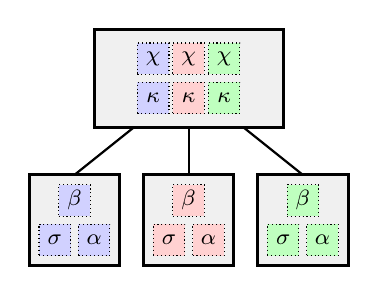
\begin{tikzpicture}
    \node[thickhost,minimum width=24mm,minimum height=12.5mm] at (1.3,0.2) {};
    \foreach \x/\c in {0.85/pdA, 1.3/pdB, 1.75/pdC} {
      \node[pdcomp=\c] at (\x,0.45) {$\chi$};
      \node[pdcomp=\c] at (\x,-0.05) {$\kappa$};
    }
    \foreach \x/\c/\t in {-0.15/pdA/0.6, 1.3/pdB/1.3, 2.75/pdC/2.0} {
      \draw[hostlink] (\t,-0.425) -- (\x,-1.025);
      \node[thickhost,minimum width=11.5mm,minimum height=11.5mm] at (\x,-1.6) {};
      \node[pdcomp=\c] at (\x,-1.35) {$\beta$};
      \node[pdcomp=\c] at (\x-0.25,-1.85) {$\sigma$};
      \node[pdcomp=\c] at (\x+0.25,-1.85) {$\alpha$};
    }
  \end{tikzpicture}
  \caption{Big data in the cloud}
  \label{fig:pulverisation-deployments-cloud}
\end{subfigure}\hfill
\begin{subfigure}[b]{0.48\textwidth}
  \centering
  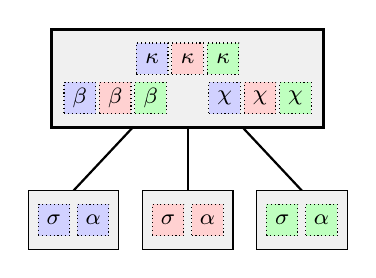
\begin{tikzpicture}
    \node[thickhost,minimum width=34.5mm,minimum height=12.5mm] at (1.3,0.2) {};
    \foreach \x/\c in {0.85/pdA, 1.3/pdB, 1.75/pdC}
      \node[pdcomp=\c] at (\x,0.45) {$\kappa$};
    \foreach \x/\c in {-0.07/pdA, 0.38/pdB, 0.83/pdC}
      \node[pdcomp=\c] at (\x,-0.05) {$\beta$};
    \foreach \x/\c in {1.77/pdA, 2.22/pdB, 2.67/pdC}
      \node[pdcomp=\c] at (\x,-0.05) {$\chi$};
    \foreach \x/\c/\t in {-0.15/pdA/0.6, 1.3/pdB/1.3, 2.75/pdC/2.0} {
      \draw[hostlink] (\t,-0.425) -- (\x,-1.225);
      \node[thinhost,minimum width=11.5mm,minimum height=7.5mm] at (\x,-1.6) {};
      \node[pdcomp=\c] at (\x-0.25,-1.6) {$\sigma$};
      \node[pdcomp=\c] at (\x+0.25,-1.6) {$\alpha$};
    }
  \end{tikzpicture}
  \caption{Thin hosts}
  \label{fig:pulverisation-deployments-thin}
\end{subfigure}

\medskip
\begin{tikzpicture}[font=\footnotesize,node distance=1mm]
  \node[thickhost,minimum width=5mm,minimum height=4mm] (k) {};
  \node[right=of k] (kt) {thick host};
  \node[thinhost,minimum width=5mm,minimum height=4mm,right=4mm of kt] (t) {};
  \node[right=of t] (tt) {thin host};
  \draw[hostlink] ([xshift=4mm]tt.east) -- ++(5mm,0) coordinate (l);
  \node[right=of l] (lt) {host-to-host link};
  \draw[neighbourlink] ([xshift=4mm]lt.east) -- ++(5mm,0) coordinate (n);
  \node[right=of n] {logical neighbour link};
\end{tikzpicture}

{\footnotesize $\sigma$ sensing \quad $\alpha$ actuation \quad $\beta$ behaviour \quad $\kappa$ state \quad $\chi$ communication\par}
